\FloatBarrier
\section{Interpolating Trajectories}
\label{sec::23_it}
As already shortly depicted in figure \ref{fig::21_pg}, we need to interpolate the trajectories that we obtain from the nonlinear model predictive control. This especially holds for the feet, since the computed results do only consider the pendulums dynamic balance with respect to the x-, and the y-position, but not for a robot that must lift its feet along the z-axis. Furthermore, the feet's movement shall be executed such that they stop moving when they are about to touch the ground. This constraint, and others, will be achieved by interpolating the feet trajectories with polynomials. In order to then match the center of mass trajectory's temporal resolution with the feet trajectories', we will upscale it under the already well-known assumption of a linear inverted pendulum. The resulting trajectories are shown in figure \ref{fig::23_ip} and will further be explained in the following. 
\begin{figure}[h!]
	\centering
	\subcaptionbox{}%
	[.4\linewidth]{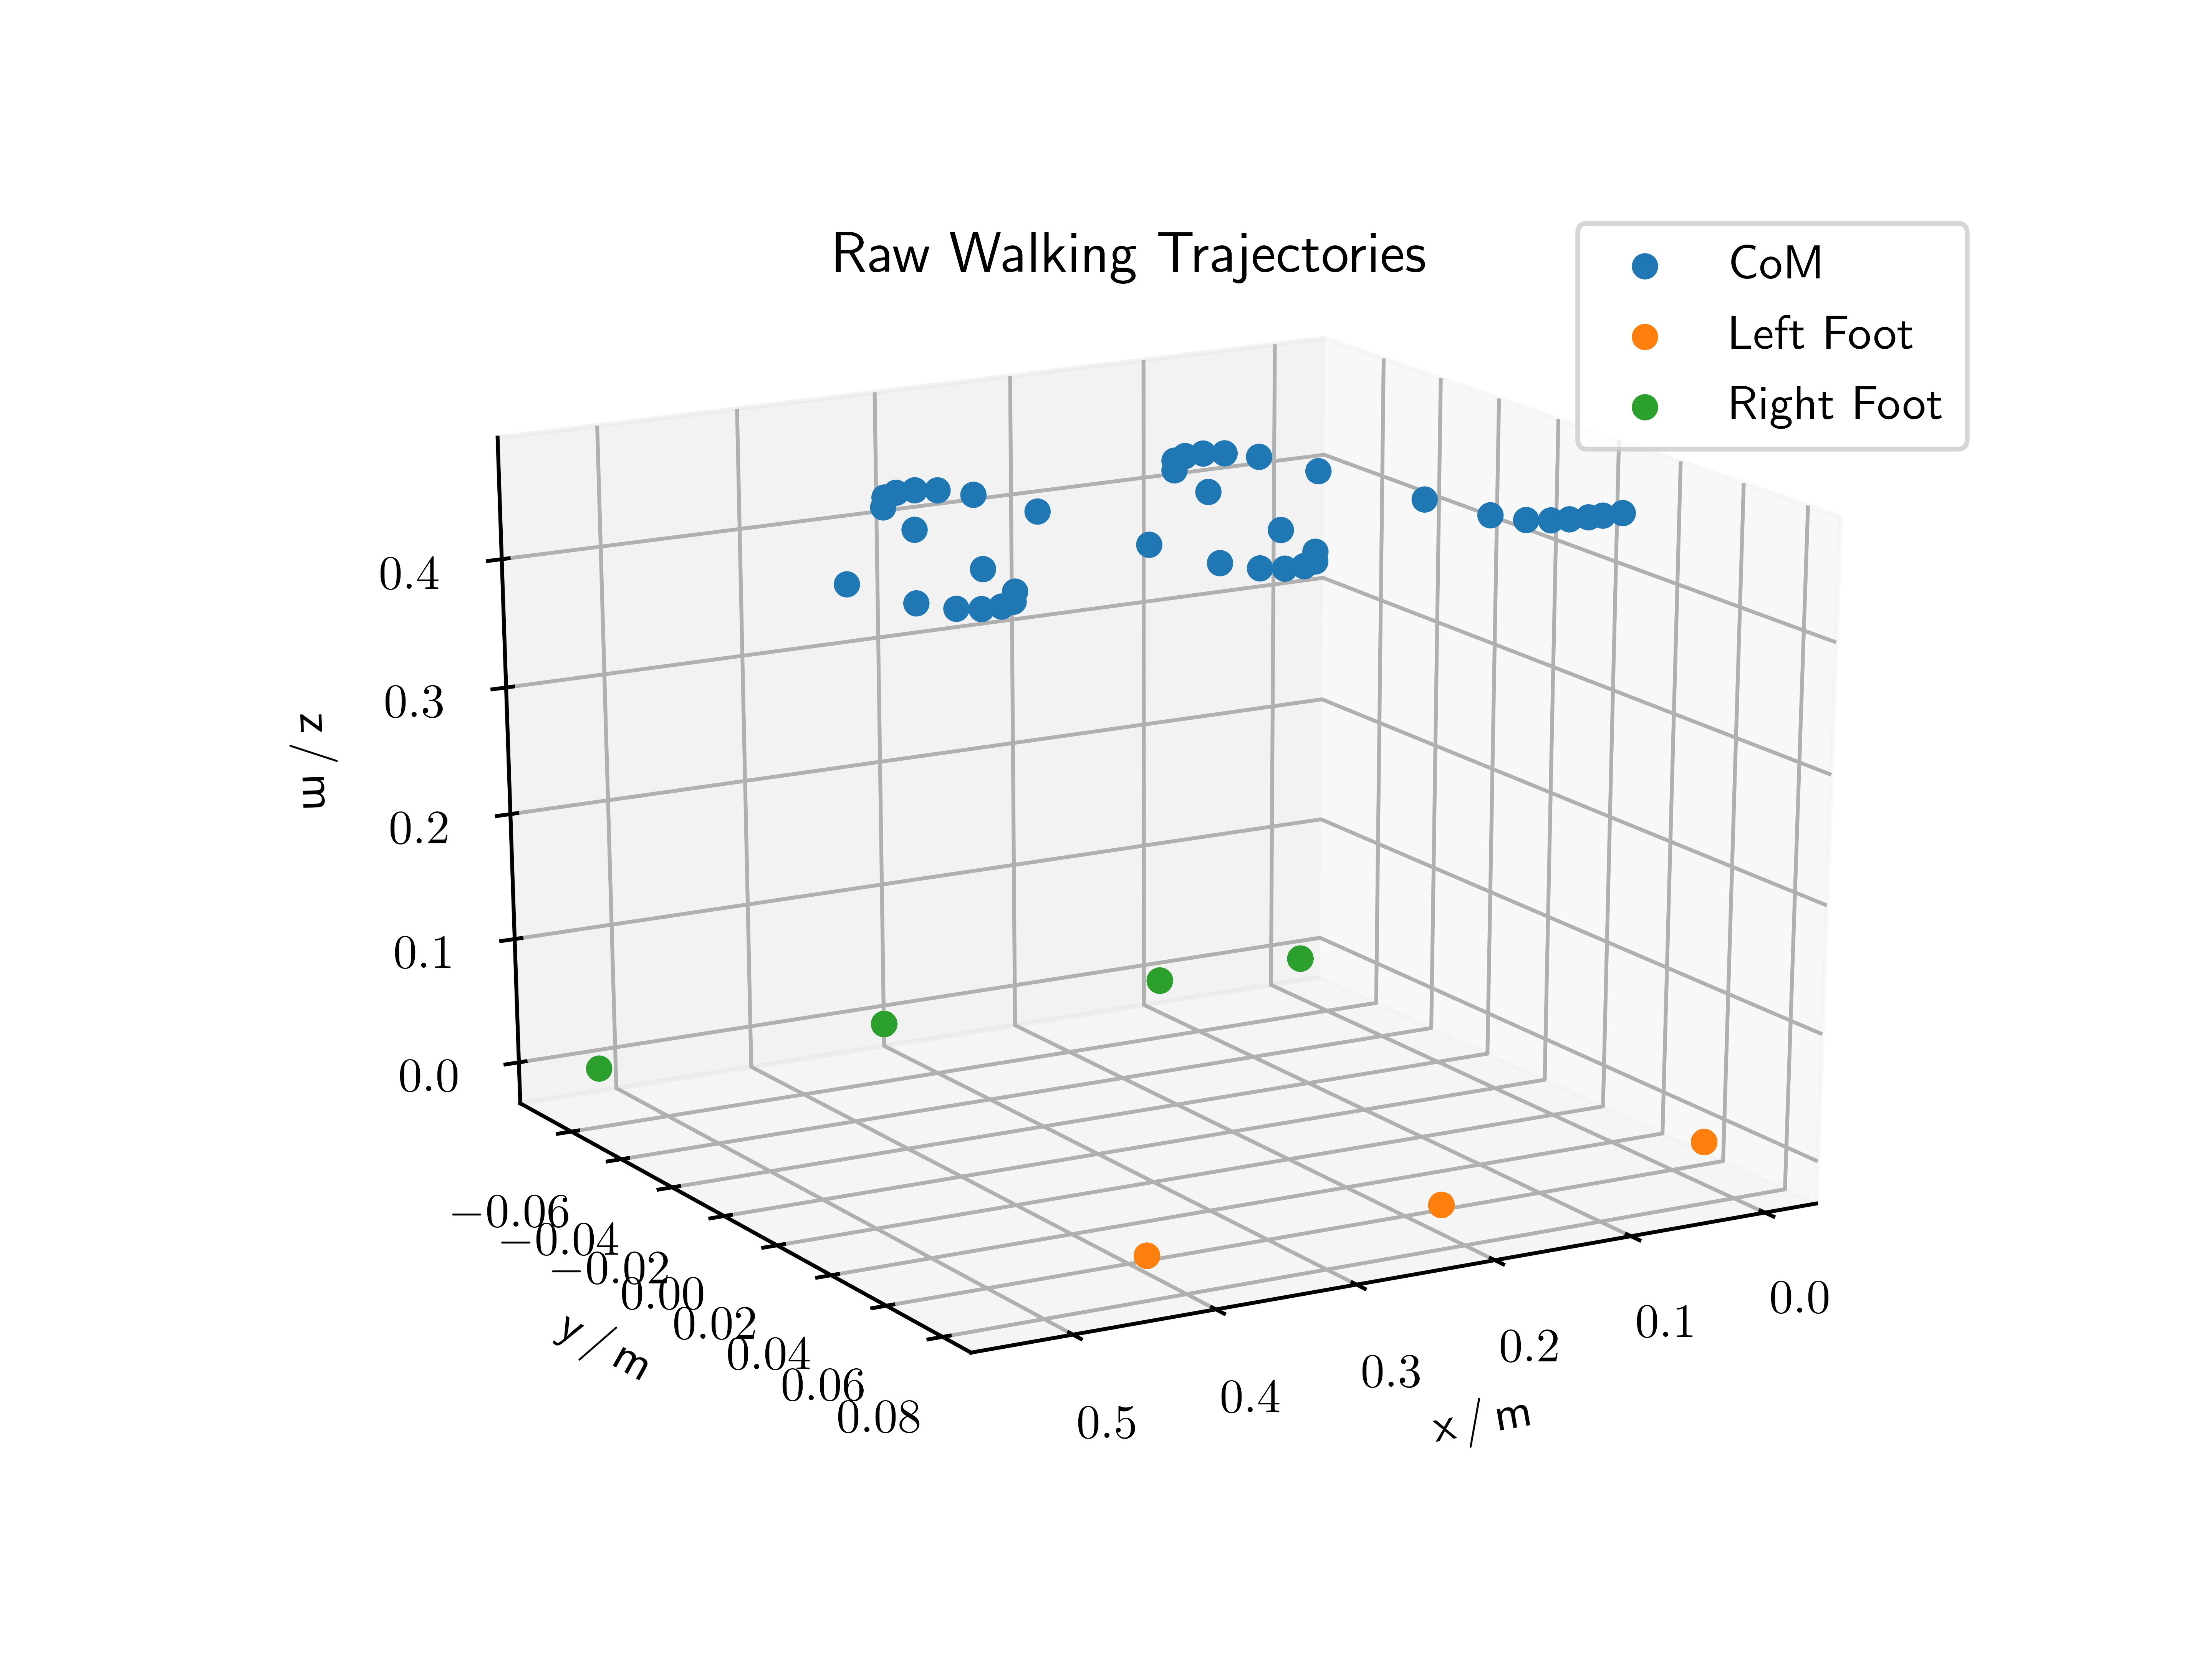
\includegraphics[scale=.4]{chapters/02_foundations_for_humanoid_walking/img/raw_results.png}}
	\subcaptionbox{}%
	[.4\linewidth]{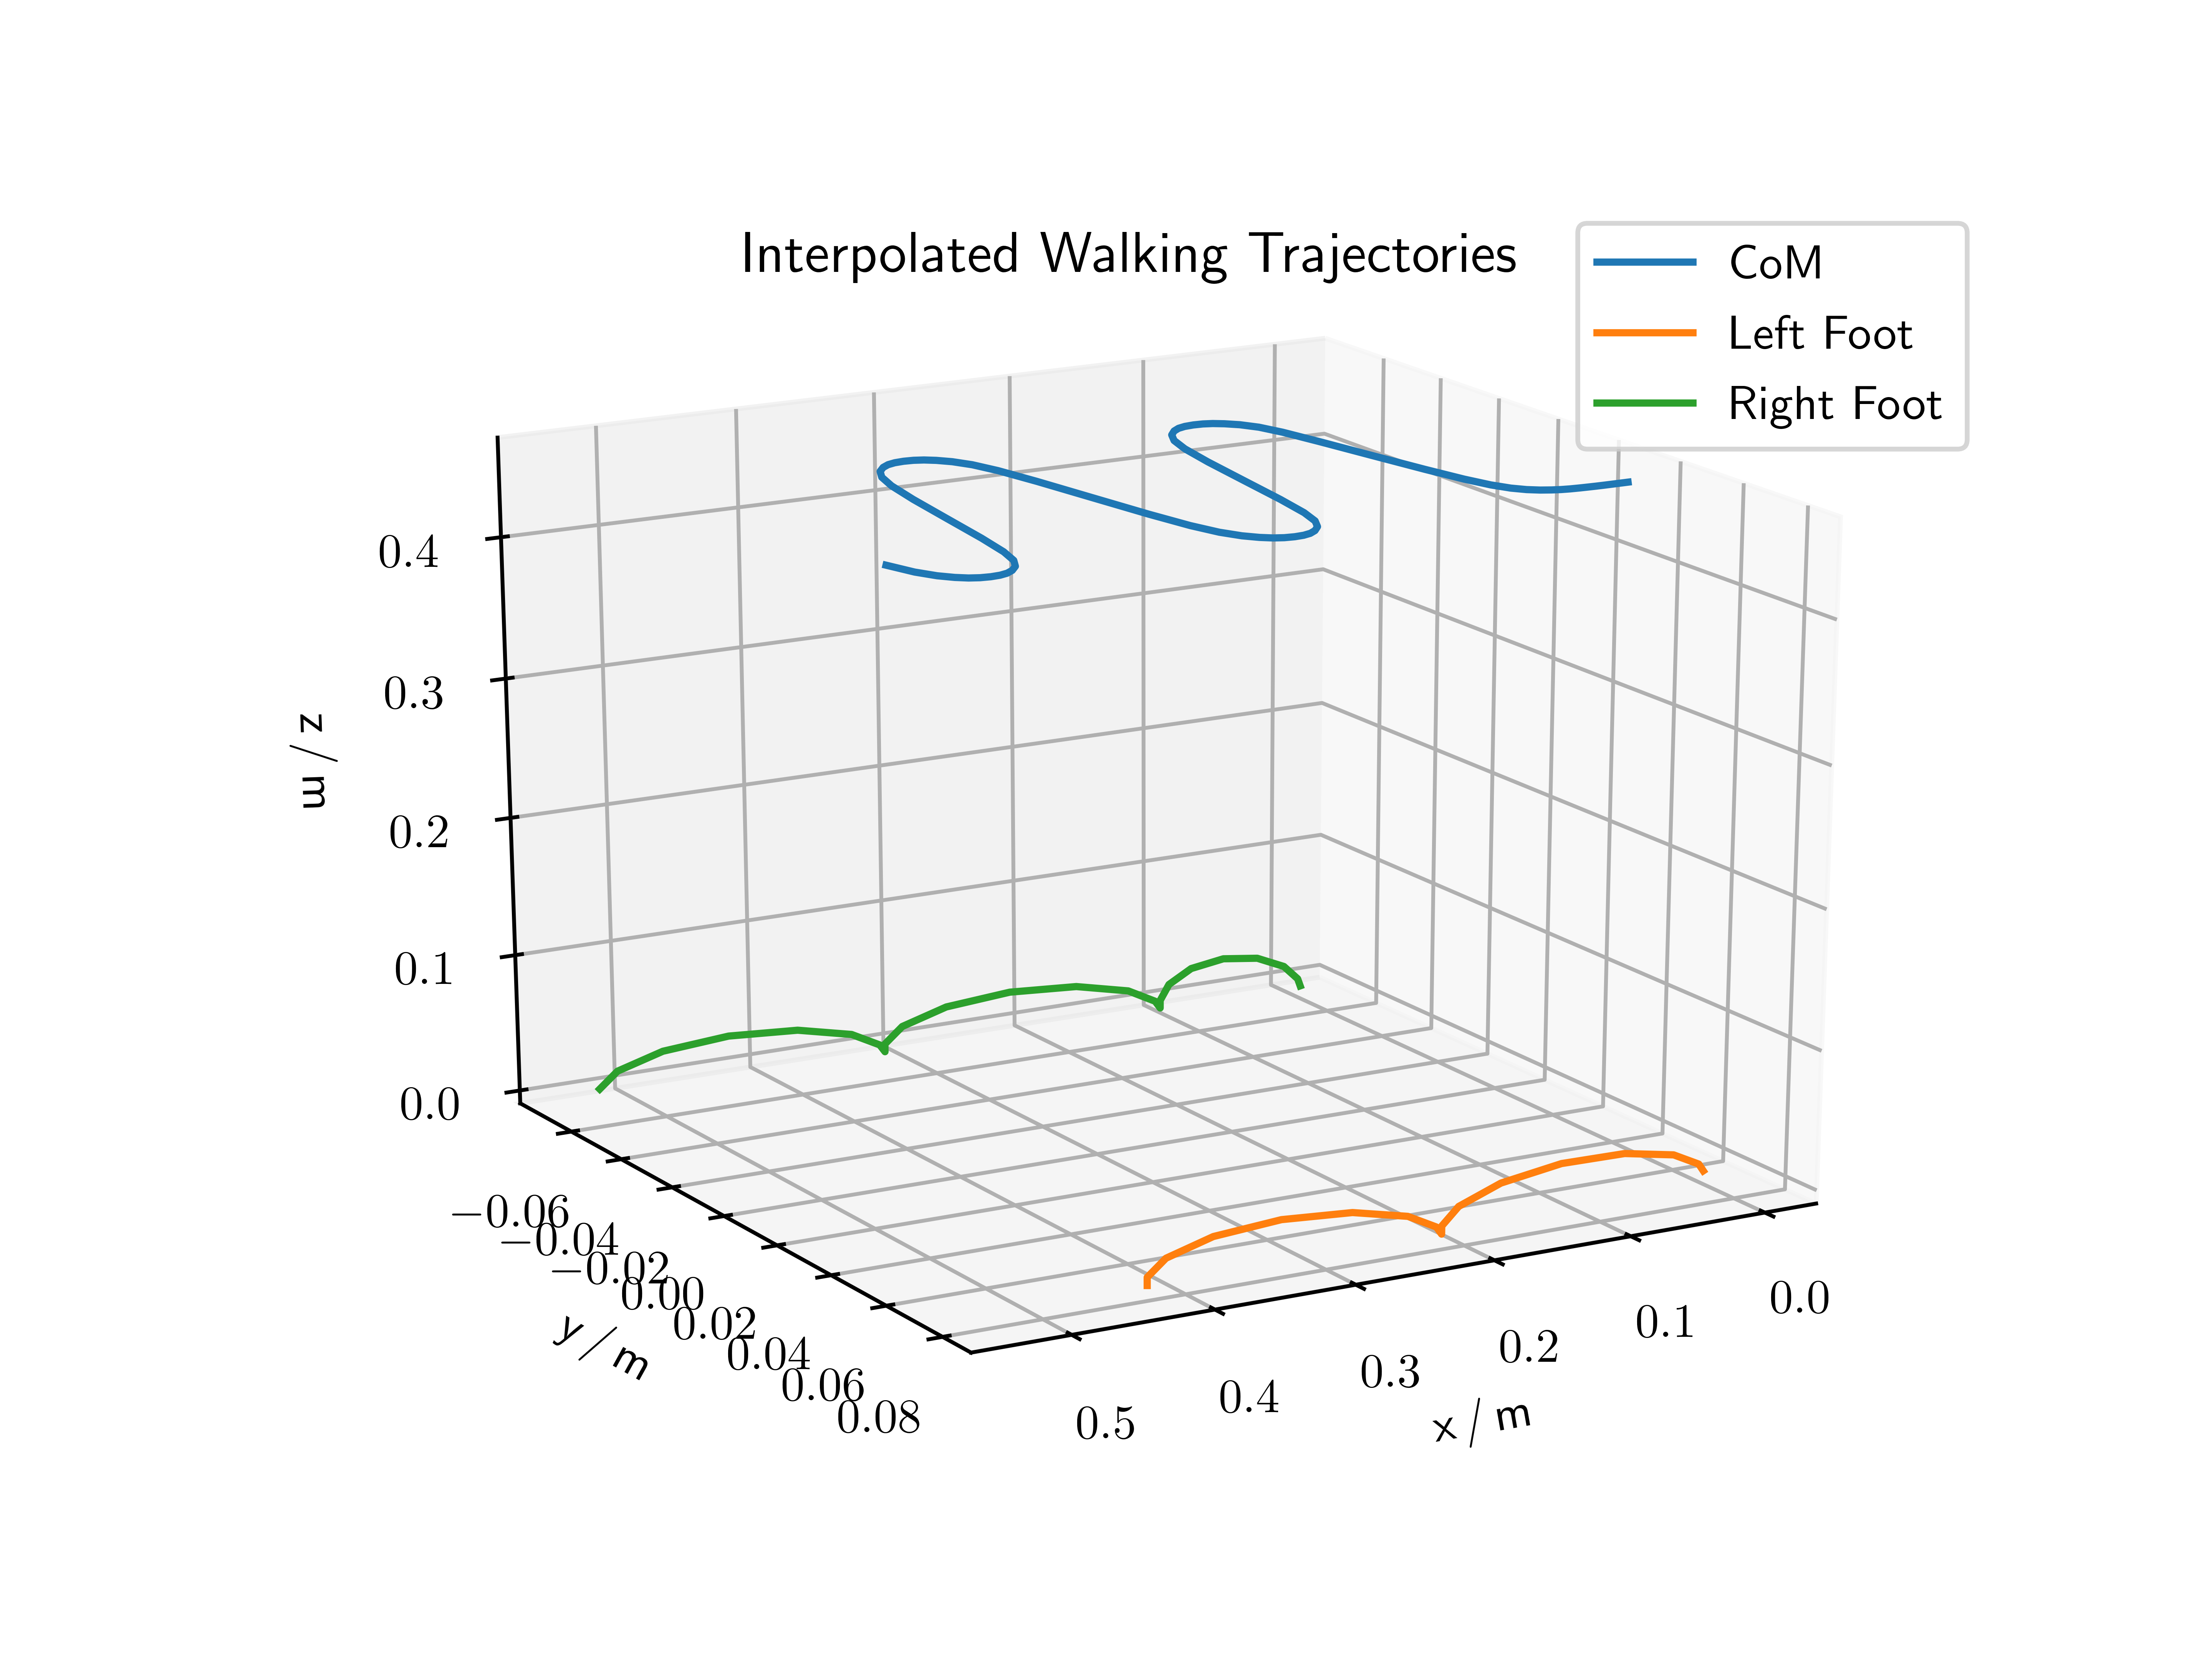
\includegraphics[scale=.4]{chapters/02_foundations_for_humanoid_walking/img/interpolated_results.png}}
	\caption{Uninterpolated trajectories (a), as obtained from the nonlinear model predictive control, and interpolated trajectories (b) for the feet and the center of mass.}
	\label{fig::23_ip}
\end{figure}
\FloatBarrier
\subsection{Interpolating the Feet Trajectories}
Any trajectory can in principal be approximated by a polynomial function. For our purposes, we want to approximate positions $p$ as they evolve over time $t$, and further obtain the corresponding velocities $\dot{p}$ and accelerations $\ddot{p}$ (equations \ref{eq::23_pos_poly} - \ref{eq::23_acc_poly}).  
\begin{align}
	p(t) &= \sum_{i = 0}^{N}a_it^i 
	\label{eq::23_pos_poly}\\
	\dot{p}(t) &= \sum_{i = 1}^{N}ia_it^{(i-1)} 
	\label{eq::23_vel_poly}\\
	\ddot{p}(t) &= \sum_{i = 2}^{N}i(i-1)a_it^{(i-2)}
	\label{eq::23_acc_poly}
\end{align}
The coefficients $a_i$ of the polynomials can be chosen such that certain boundary conditions $\bm{b}$ are satisfied. For the lift-off and the drop-down of the robot's feet, these boundary conditions must satisfy a zero initial velocity $\dot{z}_\text{init}$ and a zero end velocity $\dot{z}_\text{end}$, as well as a zero initial height $z_\text{init}$ and a zero end height $z_\text{end}$, and a maximum step height $z_{T/2}$ in between, or else they will hit the ground in an unbalanced way. These conditions are listed below, where each height $z(t)$ and each velocity $\dot{z}(t)$ is written in terms of a polynomial, just as in equations \ref{eq::23_pos_poly} and \ref{eq::23_vel_poly}, respectively. 
\begin{align}
	z(t = 0) &= z_\text{init} = 0
	\label{eq::23_z_bound_1} \\
	\dot{z}(t = 0) &= \dot{z}_\text{init} = 0 \\
	z(t = \frac{T}{2}) &= z_{T/2}
	\label{eq::23_step}\\  
	z(t = T) &= z_\text{end} = 0 \\
	\dot{z}(t = T) &= \dot{z}_\text{end} = 0 
	\label{eq::23_z_bound_5}
\end{align}
To satisfy 5 boundary conditions, it is required to have a polynomial of 4th order with 5 coefficients $a_{z,i}$ in total. In matrix formulation we can express equations \ref{eq::23_z_bound_1} - \ref{eq::23_z_bound_5} as follows
\begin{align}
	\bm{M}_z\bm{a}_z &= \bm{b}_z \\
	\begin{pmatrix}
		1 & 0 & 0              & 0              & 0 \\
		0 & 1 & 0              & 0              & 0 \\
		1 & \left(\frac{T}{2}\right)        & \left(\frac{T}{2}\right)^2  & \left(\frac{T}{2}\right)^3 & \left(\frac{T}{2}\right)^4 \\
		1 & T & T^2            & T^3            & T^4 \\
		0 & 1 & 2T             & 3T^2           & 4T^3 
	\end{pmatrix}
	\begin{pmatrix}
		a_{z,0} \\
		a_{z,1} \\
		a_{z,2} \\
		a_{z,3} \\
		a_{z,4}
	\end{pmatrix} &=
	\begin{pmatrix}
		z_\text{init} \\
		\dot{z}_\text{init} \\
		z_{T/2} \\
		z_\text{end}\\
		\dot{z}_\text{end}
	\end{pmatrix}.
\end{align}
Inversion then yields
\begin{align}
	\bm{a}_z&=\bm{M}_z^{-1}\bm{b}_z \\
	\begin{pmatrix}
		a_{z,0} \\
		a_{z,1} \\
		a_{z,2} \\
		a_{z,3} \\
		a_{z,4}
	\end{pmatrix} &=
	\begin{pmatrix}
		1 & 0 & 0 & 0 & 0 \\
		0 & 1 & 0 & 0 & 0 \\
		-\frac{11}{T^2} & -\frac{4}{T} & \frac{16}{T^2} & -\frac{5}{T^2} & \frac{1}{T} \\
		\frac{18}{T^3} & \frac{5}{T^2} & -\frac{32}{T^3} & \frac{14}{T^3} & -\frac{3}{T^2} \\
		-\frac{8}{T^4} & -\frac{2}{T^3} & \frac{16}{T^4} & -\frac{8}{T^4} & \frac{2}{T^3}
	\end{pmatrix}
	\begin{pmatrix}
		z_\text{init} \\
		\dot{z}_\text{init} \\
		z_{T/2} \\
		z_\text{end}\\
		\dot{z}_\text{end}
	\end{pmatrix}.
\end{align}
The obtained coefficients $a_i$ are then used to compute the height of each foot during a single support phase (\href{https://github.com/mhubii/nmpc_pattern_generator/blob/c82c64a28da7527e75442764f585bd50a8f61ee9/libs/pattern_generator/src/interpolation.cpp#L779}{\underline{link}}). The maximum step height $z_{T/2}$ (\href{https://github.com/mhubii/nmpc_pattern_generator/blob/c82c64a28da7527e75442764f585bd50a8f61ee9/libs/pattern_generator/configs.yaml#L22}{\underline{link}}), and the single support time $T$ (\href{https://github.com/mhubii/nmpc_pattern_generator/blob/c82c64a28da7527e75442764f585bd50a8f61ee9/libs/pattern_generator/configs.yaml#L21}{\underline{link}}), which is the step time minus the double support time, can be set in the configurations file. For the x-, and the y-positions of the feet, we can define boundary conditions in a similar fashion. In contrary to the computation of the z-position, the x-, and the y-position interpolation of the feet allows for feedback. Therefore, we require additional constraints that satisfy the accelerations as follows
\begin{align}
	x(t = 0) &= x_\text{init} 
	\label{eq::23_x_bound_1}\\
	\dot{x}(t=0) &= \dot{x}_\text{init} \\
	\ddot{x}(t=0) &= \ddot{x}_\text{init} \\
	x(t=T) &= x_\text{end}\\
	\dot{x}(t=T) &= \dot{x}_\text{end} \\
	\ddot{x}(t=T) &= \ddot{x}_\text{end}.
	\label{eq::23_x_bound_6}
\end{align}
Again, we can rewrite equations \ref{eq::23_x_bound_1} - \ref{eq::23_x_bound_6} in matrix formulation
\begin{align}
	\bm{M}_x\bm{a}_x &= \bm{b}_x \\
	\begin{pmatrix}
		1 & 0 & 0 & 0 & 0 & 0 \\
		0 & 1 & 0 & 0 & 0 & 0 \\
		0 & 0 & 2 & 0 & 0 & 0 \\
		1 & T & T^2 & T^3 & T^4 & T^5 \\
		0 & 1 & 2 T & 3 T^2 & 4 T^3 & 5 T^4 \\
		0 & 0 & 2 & 6 T & 12 T^2 & 20 T^3
	\end{pmatrix}
	\begin{pmatrix}
		a_{x,0} \\
		a_{x,1} \\
		a_{x,2} \\
		a_{x,3} \\
		a_{x,4} \\
		a_{x,5}
	\end{pmatrix} &=
	\begin{pmatrix}
		x_\text{init} \\
		\dot{x}_\text{init} \\
		\ddot{x}_\text{init} \\
		x_\text{end} \\
		\dot{x}_\text{end} \\
		\ddot{x}_\text{end} 
	\end{pmatrix},
\end{align}
and inversion yields the polynomial's coefficients $a_{x,i}$
\begin{align}
	\bm{a}_x &= \bm{M}_x^{-1}\bm{b}_x \\
	\begin{pmatrix}
		a_{x,0} \\
		a_{x,1} \\
		a_{x,2} \\
		a_{x,3} \\
		a_{x,4} \\
		a_{x,5}
	\end{pmatrix} &= 
	\frac{1}{2}
	\begin{pmatrix}
		2 & 0 & 0 & 0 & 0 & 0 \\
		0 & 2 & 0 & 0 & 0 & 0 \\
		0 & 0 & 1 & 0 & 0 & 0 \\
		-\frac{20}{T^3} & -\frac{12}{T^2} & -\frac{3}{T} & \frac{20}{T^3} & -\frac{8}{T^2} & \frac{1}{T} \\
		\frac{30}{T^4} & \frac{16}{T^3} & \frac{3}{T^2} & -\frac{30}{T^4} & \frac{14}{T^3} & -\frac{2}{T^2} \\
		-\frac{12}{T^5} & -\frac{6}{T^4} & -\frac{1}{T^3} & \frac{12}{T^5} & -\frac{6}{T^4} & \frac{1}{T^3} \\
	\end{pmatrix}
	\begin{pmatrix}
		x_\text{init} \\
		\dot{x}_\text{init} \\
		\ddot{x}_\text{init} \\
		x_\text{end} \\
		\dot{x}_\text{end} \\
		\ddot{x}_\text{end} 
	\end{pmatrix}.
\end{align}
The exact same formalism is used to interpolate the foot's y-position during single support phase (\href{https://github.com/mhubii/nmpc_pattern_generator/blob/c82c64a28da7527e75442764f585bd50a8f61ee9/libs/pattern_generator/src/interpolation.cpp#L806}{\underline{link}}). In contrast to the interpolation of the feet's positions, the center of mass positions will be extrapolated under the introduced assumption of a linear inverted pendulum. The method will be shortly explained in the following paragraph - Interpolating the Center of Mass Trajectories.
\FloatBarrier
\subsection{Interpolating the Center of Mass Trajectories}
The center of mass trajectories can now simply be adjusted to the temporal resolution of the feet trajectories by applying the linear time-stepping scheme from equation \ref{eq::223_ltss} with an adjusted temporal resolution $T$. An iterative application (\href{https://github.com/mhubii/nmpc_pattern_generator/blob/5a213044c927dc6aac9f7e32ce1e5fb472cd67bb/libs/pattern_generator/src/interpolation.cpp#L776}{\underline{link}}) of these matrices then yields the desired interpolation. The only requirement left to get our robot to walk is now the transformation of trajectories in Cartesian space to trajectories within the joint space, which will be resolved in the following chapter - Kinematics.